% ============================================================
%  DEOS Algoritmalari -- Teknik Dokumantasyon
%  TEKNOFEST 2026 Robotaksi-Binek Ozerk Arac Yarismasi
% ============================================================
\documentclass[a4paper,12pt]{article}

\usepackage[utf8]{inputenc}
\usepackage[T1]{fontenc}
\usepackage{geometry}
\usepackage{amsmath}
\usepackage{amssymb}
\usepackage{booktabs}
\usepackage{longtable}
\usepackage{array}
\usepackage{xcolor}
\usepackage{listings}
\usepackage{hyperref}
\usepackage{enumitem}
\usepackage{fancyhdr}
\usepackage{multirow}
\usepackage{tcolorbox}
\usepackage{tikz}
\usetikzlibrary{shapes.geometric, arrows.meta, positioning}

\geometry{
  left=2.5cm, right=2.5cm,
  top=2.5cm,  bottom=2.5cm
}

\hypersetup{
  colorlinks=true,
  linkcolor=blue!70!black,
  urlcolor=blue!60!black,
}

\definecolor{codebg}{rgb}{0.96,0.96,0.96}

\lstset{
  basicstyle=\ttfamily\small,
  keywordstyle=\color{blue!70!black}\bfseries,
  commentstyle=\color{green!50!black}\itshape,
  stringstyle=\color{red!60!black},
  numbers=left,
  numberstyle=\tiny\color{gray},
  numbersep=6pt,
  backgroundcolor=\color{codebg},
  frame=single,
  breaklines=true,
  tabsize=4,
  language=Python,
  showstringspaces=false,
  xleftmargin=1.8em
}

\tcbuselibrary{most}

\newtcolorbox{notebox}[1][]{
  colback=blue!5,
  colframe=blue!40!black,
  fonttitle=\bfseries,
  title=Not,
  #1
}

\newtcolorbox{specbox}[1][]{
  colback=green!5,
  colframe=green!45!black,
  fonttitle=\bfseries,
  title=Sartname Gerekliligi,
  #1
}

\newtcolorbox{warnbox}[1][]{
  colback=orange!8,
  colframe=orange!70!black,
  fonttitle=\bfseries,
  title=Dikkat,
  #1
}

\pagestyle{fancy}
\fancyhf{}
\rhead{DEOS Algoritmalari}
\lhead{TEKNOFEST 2026}
\cfoot{\thepage}

\title{
  \vspace{-1cm}
  \textbf{\LARGE DEOS Algoritmalari}\\[0.4em]
  \large Teknik Dokumantasyon\\[0.2em]
  \normalsize TEKNOFEST 2026 Robotaksi-Binek Ozerk Arac Yarismasi\\[0.2em]
  \normalsize \texttt{deos\_algorithms} paketi --- \today
}
\author{BurakSahin00 / DEOS Takim}
\date{}

\begin{document}
\maketitle
\tableofcontents
\newpage

% ============================================================
\section{Giris ve Mimari Genel Bakis}
% ============================================================

\subsection{Amac}

\texttt{deos\_algorithms} paketi, TEKNOFEST 2026 Robotaksi-Binek Ozerk Arac
Yarismasi icin gelistirilmis \textbf{saf Python} algoritma katmanidir. Bu
katman:

\begin{itemize}
  \item ROS 2 mesajlarindan tamamen bagimsizdir; birim test edilebilir,
  \item Her modul \emph{durum makinesi} veya \emph{durumsuz fonksiyon} olarak
        tasarlanmistir,
  \item Yarismada puanlanacak her senaryo icin ayri bir modul bulunmaktadir.
\end{itemize}

\subsection{Modul Hiyerarsisi}

\begin{center}
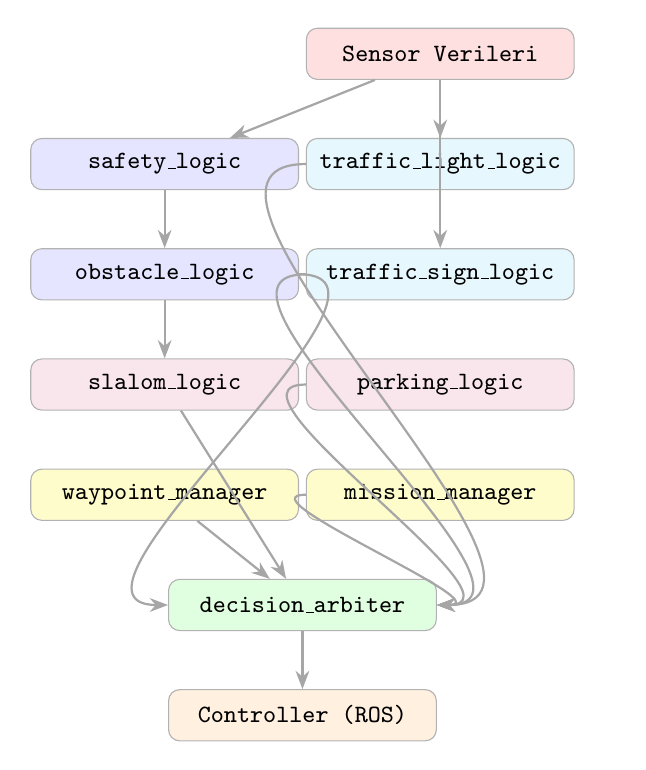
\begin{tikzpicture}[
  box/.style={
    rectangle, draw=gray!60, rounded corners=4pt,
    minimum width=3.4cm, minimum height=0.65cm,
    font=\small\ttfamily, text centered, fill=white
  },
  arrow/.style={-Stealth, thick, gray!70}
]

% --- Row 0: sensor input ---
\node[box, fill=red!12]  (sensor) at (4.0, 0)   {Sensor Verileri};

% --- Row 1: perception ---
\node[box, fill=blue!10] (safety) at (0.5,-1.4) {safety\_logic};
\node[box, fill=blue!10] (obs)    at (0.5,-2.8) {obstacle\_logic};
\node[box, fill=cyan!10] (light)  at (4.0,-1.4) {traffic\_light\_logic};
\node[box, fill=cyan!10] (sign)   at (4.0,-2.8) {traffic\_sign\_logic};
\node[box, fill=purple!10](slalom)at (0.5,-4.2) {slalom\_logic};
\node[box, fill=purple!10](park)  at (4.0,-4.2) {parking\_logic};

% --- Row 2: planning ---
\node[box, fill=yellow!20](wp)    at (0.5,-5.6) {waypoint\_manager};
\node[box, fill=yellow!20](mm)    at (4.0,-5.6) {mission\_manager};

% --- Row 3: arbiter ---
\node[box, fill=green!12] (arb)   at (2.25,-7.0){decision\_arbiter};

% --- Row 4: output ---
\node[box, fill=orange!12](ctrl)  at (2.25,-8.4){Controller (ROS)};

% Arrows
\draw[arrow] (sensor) -- (safety);
\draw[arrow] (sensor) -- (light);
\draw[arrow] (sensor) -- (sign);
\draw[arrow] (safety) -- (obs);
\draw[arrow] (obs)    -- (slalom);
\draw[arrow] (obs)    to[out=0,in=180] (arb);
\draw[arrow] (light)  to[out=180,in=0] (arb);
\draw[arrow] (sign)   to[out=180,in=0] (arb);
\draw[arrow] (slalom) -- (arb);
\draw[arrow] (park)   to[out=180,in=0] (arb);
\draw[arrow] (wp)     -- (arb);
\draw[arrow] (mm)     to[out=180,in=0] (arb);
\draw[arrow] (arb)    -- (ctrl);

\end{tikzpicture}
\end{center}

\subsection{Temel Tasarim Prensipleri}

\begin{enumerate}
  \item \textbf{ROS bagimsizligi:} Hicbir modul \texttt{rclpy} veya ROS mesaj
        tipi icermez. Tipler saf Python \texttt{dataclass}'lardir.
  \item \textbf{Deterministik oncelik:} \texttt{decision\_arbiter} tum ciktilari
        sabit bir oncelik sirasina gore bilestirir.
  \item \textbf{Zaman bagimsizligi:} Zamanlayicilar \texttt{time.monotonic()}
        ile olculur; ROS Hz'inden bagimsiz calisirlar.
  \item \textbf{Tek kaynak hakikati:} Sabitler yalnizca bir modulde tanimlanir
        ve diger moduller oradan iceri aktarir.
\end{enumerate}

% ============================================================
\section{Guvenlik Modulu (\texttt{safety\_logic.py})}
% ============================================================

\subsection{Amac ve Kapsam}

\texttt{SafetyLogic}, her goruntu karesinde gelen nesne tespit kutularini
(BBox) alarak aracin anlik tehdit duzeyini ve hiz tavanini hesaplar. Bu modul
diger tum kararlarin \emph{tabanini} olusturur; \texttt{obstacle\_logic}
bu modulu icsellestirir.

\subsection{Koridor Modeli}

Arac koordinat cercevesinde ileri yonunde dikdortgen bir guvenlik koridoru:

\begin{align}
  \text{Koridor genisligi} &= 2 \times 1{,}2\text{ m} = 2{,}4\text{ m}\\
  \text{Koridor uzunlugu} &= 20{,}0\text{ m}
\end{align}

\begin{notebox}
Koridora giren nesne: $|lateral\_m| \leq 1{,}2$ ve $0 < dist \leq 20{,}0$ m.
Disindaki nesneler tehdit olarak degerlendirilmez.
\end{notebox}

\subsection{Mesafe Tahmini}

Harici derinlik (stereo/LiDAR) yoksa bbox pin-hole formuluyle tahmin edilir:

\begin{equation}
  d = \frac{h_{cam} \cdot f_{px}}{v - v_{pp}}
\end{equation}

$h_{cam}=1{,}2$ m, $f_{px}=800$ px, $v$ bbox alt merkezinin piksel
y-koordinati, $v_{pp}=240$ px (ana nokta, 480 px yuksekliginin yarisi).

Yanal ofset (pozitif = sol, negatif = sag):
\begin{equation}
  lateral = -\frac{(u - W/2) \cdot d}{f_{px}}
\end{equation}

\subsection{Sinif Temkinlilik Carpanlari}

\begin{center}
\begin{tabular}{lcc}
  \toprule
  Sinif            & Carpan ($c$) & Etkin mesafe\\
  \midrule
  Yaya             & 1.5          & $d / 1{,}5$\\
  Arac             & 1.2          & $d / 1{,}2$\\
  Koni / Bariyer   & 1.0          & $d$\\
  Bilinmeyen       & 1.3          & $d / 1{,}3$\\
  \bottomrule
\end{tabular}
\end{center}

Etkin mesafe $d_{eff} = d / c$ ile hesaplanir; yaya 6 m'de bir arac kadar
tehditkar gorunur.

\subsection{Tehdit Bantlari}

\begin{center}
\begin{tabular}{llcl}
  \toprule
  Bant        & Esik ($d_{eff}$)     & Hiz tavan & Karar\\
  \midrule
  Acil dur    & $< 3{,}0$ m           & 0.0        & \texttt{emergency\_stop=True}\\
  Sert yavas  & $< 8{,}0$ m           & 0.5        & \texttt{HARD\_SLOW}\\
  Yumus yavas & $< 15{,}0$ m          & 0.8        & \texttt{SOFT\_SLOW}\\
  Guvenli     & $\geq 15{,}0$ m       & 1.0        & \texttt{NONE}\\
  \bottomrule
\end{tabular}
\end{center}

\subsection{Nesne Takipci (SimpleTracker)}

Sahte alarm gidermek icin merkez-mesafesi tabanli tracker:

\begin{itemize}
  \item Eslestirme: Okalipya mesafesi $< 80$ px olan iz secilir.
  \item Onaylama: $\geq 3$ ardisik kare gorulunce iz ``onaylandi''.
  \item Silme: $\geq 5$ kare gorulmeyince iz silinir.
\end{itemize}

Sadece \textbf{onaylanmis} izler tehdit olarak degerlendirilir.

% ============================================================
\section{Engel Mantigi (\texttt{obstacle\_logic.py})}
% ============================================================

\subsection{Amac}

\texttt{ObstacleLogic}, \texttt{SafetyLogic} uzerinde ikinci bir katman olarak
\emph{dinamik} (yaya) ve \emph{statik} (koni, bariyer) engeller icin ayri
davranis politikalari uretir.

\subsection{Engel Siniflandirmasi}

\begin{center}
\begin{tabular}{ll}
  \toprule
  Sinif               & Kabul edilen sinif adlari\\
  \midrule
  \texttt{PEDESTRIAN} & pedestrian, person, people, yaya, insan\\
  \texttt{CONE}       & cone, traffic\_cone, koni\\
  \texttt{BARRIER}    & barrier, fence, roadblock, bariyer, engel\\
  \bottomrule
\end{tabular}
\end{center}

\subsection{Dinamik Engel Davranisi}

\begin{specbox}
Sartname Tur-2/Tur-3: Dinamik engelden (yaya) basariyla sakinmak 50 puan.
\end{specbox}

\textbf{Uc asama:}
\begin{enumerate}
  \item \textbf{SLOW} ($\leq 10$ m): Hiz tavan $\min(cap, 0{,}4)$.
  \item \textbf{WAIT} ($\leq 5$ m): Tam dur. $\geq 3$ ardisik bos kare
        gorunce bekleme sona erer.
  \item \textbf{AVOID\_AFTER\_STOP:} \texttt{DYNAMIC\_AVOID\_HOLD\_S = 0{,}4 s}
        bekledikten sonra $|lat| \geq 0{,}35$ m ise karsit yonden gecis onerisi:
        \begin{itemize}
          \item $lat > 0$ (engel sol) $\Rightarrow$ \texttt{direction=''right''}
          \item $lat < 0$ (engel sag) $\Rightarrow$ \texttt{direction=''left''}
        \end{itemize}
\end{enumerate}

\subsection{Statik Engel Davranisi}

\begin{specbox}
Sartname Tur-1/Tur-3: Statik engelden basariyla sakinmak 50 puan.
\end{specbox}

\begin{itemize}
  \item $dist \leq 3{,}0$ m: Yavaslatir (\texttt{speed\_cap = 0{,}35}).
  \item \textbf{Yon karari:} $lat \geq 0$ (engel sol) $\Rightarrow$ sagdan
        gec; $lat < 0$ (engel sag) $\Rightarrow$ soldan gec.
  \item \textbf{Commit mekanizmasi:} Ardisik konilerde zigzag onlemek icin yon
        6 kare boyunca kilitlenir. Zit tarafa gecis icin mesafe farki
        $\geq 0{,}6$ m olmalidir.
  \item $> 1$ bariyer gorulurse \texttt{road\_blocked=True}: planlayici
        alternatif rota hesaplar.
\end{itemize}

% ============================================================
\section{Trafik Isigi Mantigi (\texttt{traffic\_light\_logic.py})}
% ============================================================

\subsection{Amac}

Kamera tabanli trafik isigi tespitlerini (kirmizi/sari/yesil) durum
makinesiyle degerlendirip aracin hizi ve hareket iznine donusturur.

\begin{specbox}
Puan Tablosu (sartname):\\
Yesil isikta $\leq 5$ sn harekete gecme: \textbf{+40 p}\\
Yesil isikta 5--30 sn harekete gecme: \textbf{+20 p}\\
Yesil isikta $>30$ sn: \textbf{$-$20 p}\\
Kirmizi isikta gec: \textbf{$-$30 p}
\end{specbox}

\subsection{Renk Tespiti ve Onaylama}

\begin{itemize}
  \item Minimum guven: \texttt{MIN\_CONFIDENCE = 0.45}
  \item Onaylama: $\geq 2$ ardisik kare (\texttt{CONFIRM\_FRAMES = 2})
  \item Gecerlilik: 1.5 saniye gorulmezse hafizadan silinir
\end{itemize}

\subsection{Karar Kurallari}

\begin{center}
\begin{tabular}{lll}
  \toprule
  Aktif renk               & Kosal         & Karar\\
  \midrule
  Kirmizi                  & $d \leq 3$ m  & \texttt{must\_stop=True, cap=0.0}\\
  Kirmizi                  & $3 < d \leq 8$ m & \texttt{cap=0.5}\\
  Kirmizi                  & $8 < d \leq 15$ m & \texttt{cap=0.8}\\
  Sari (kirmizi sonrasi)   & hareket halinde   & \texttt{prepare\_to\_move, cap=0.25}\\
  Sari (diger)             & hareket halinde   & \texttt{prepare\_to\_stop, cap=0.4}\\
  Yesil                    & ---               & \texttt{can\_go=True}\\
  \bottomrule
\end{tabular}
\end{center}

\subsection{Yesil Isik Tepki Suresi Takibi}

Sartname puan kademelerini desteklemek icin, yesil isik ilk onaylandiginda
zaman damgasi kaydedilir:

\begin{lstlisting}[language=Python, caption=Green timer (update metodu)]
if LightColor.GREEN in active_colors:
    if self._green_started_at is None:
        self._green_started_at = now
else:
    self._green_started_at = None
\end{lstlisting}

\texttt{TrafficLightState.green\_elapsed\_s} alani controller'a aktarilir:
\begin{align*}
  green\_elapsed\_s \leq 5 &\Rightarrow +40 \text{ p}\\
  5 < green\_elapsed\_s \leq 30 &\Rightarrow +20 \text{ p}\\
  green\_elapsed\_s > 30 &\Rightarrow -20 \text{ p}
\end{align*}

% ============================================================
\section{Trafik Tabelasi Mantigi (\texttt{traffic\_sign\_logic.py})}
% ============================================================

\subsection{Amac ve Felsefe}

Bu modul tabelalar\i{} \emph{tespit ETMEZ}; tespit edildigini varsayar.
KISIT uretir --- waypoint yoneticisi ve controller bu kisitlari
gozonunde bulundurarak kendi kararlarini verir.

\begin{specbox}
Sartname: 22 tabela sinifi tanimlidir.
Dogru tepki: +50 p. Yanlis tepki: $-$50 p.
\end{specbox}

\subsection{Desteklenen 22 Tabela Sinifi}

\begin{center}
\renewcommand{\arraystretch}{1.15}
\begin{longtable}{llp{5.0cm}}
  \toprule
  Sinif Kodu                   & Deger               & Davranis\\
  \midrule
  \endhead
  \texttt{STOP}                & dur tabelasi        & 5 sn bekle, cooldown\\
  \texttt{NO\_ENTRY}           & girilmez            & dur + \texttt{entry\_blocked=True}\\
  \texttt{PEDESTRIAN\_CROSSING}& yaya gecidi         & hiz tavan 0.5\\
  \texttt{BUS\_STOP}           & durak               & pass (mission planner islemi)\\
  \texttt{NO\_RIGHT\_TURN}     & saga donulmez       & \texttt{right=False}\\
  \texttt{NO\_LEFT\_TURN}      & sola donulmez       & \texttt{left=False}\\
  \texttt{KEEP\_RIGHT}         & sagdan gidiniz      & \texttt{forced=''pass\_right''}\\
  \texttt{KEEP\_LEFT}          & soldan gidin        & \texttt{forced=''pass\_left''}\\
  \texttt{MUST\_RIGHT}         & saga mecburi        & \texttt{forced=''right''}\\
  \texttt{MUST\_LEFT}          & sola mecburi        & \texttt{forced=''left''}\\
  \texttt{MUST\_STRAIGHT}      & ileri mecburi       & \texttt{forced=''straight''}\\
  \texttt{STRAIGHT\_OR\_RIGHT} & ileri ve saga mec.  & \texttt{right+straight}\\
  \texttt{STRAIGHT\_OR\_LEFT}  & ileri ve sola mec.  & \texttt{left+straight}\\
  \texttt{AHEAD\_THEN\_RIGHT}  & ileriden saga       & \texttt{forced=''right''}\\
  \texttt{AHEAD\_THEN\_LEFT}   & ileriden sola       & \texttt{forced=''left''}\\
  \texttt{ROUNDABOUT}          & doner kavsak        & \texttt{forced=''roundabout''}\\
  \texttt{LANE\_ARRANGEMENT\_H}& sol seridin sonu    & tur kisiti\\
  \texttt{LANE\_ARRANGEMENT\_I}& sag seridin sonu    & tur kisiti\\
  \texttt{TWO\_WAY}            & iki yonlu yol       & \texttt{two\_way\_road=True}, cap 0.6\\
  \texttt{PARKING\_AREA}       & park                & \texttt{current\_area\_is\_parking}\\
  \texttt{NO\_PARKING}         & park yapilmaz       & \texttt{current\_area\_no\_parking}\\
  \texttt{TRAFFIC\_LIGHT\_AHEAD}& isikli isaret      & \texttt{traffic\_light\_expected}\\
  \texttt{TUNNEL}              & tunel               & \texttt{approaching\_tunnel}, cap 0.7\\
  \bottomrule
\end{longtable}
\end{center}

\subsection{Onaylama ve Bellek Mekanizmasi}

\begin{itemize}
  \item Minimum guven: \texttt{MIN\_CONFIDENCE = 0.7}
  \item Onaylama: $\geq 3$ kare (\texttt{CONFIRM\_FRAMES = 3})
  \item Gecerlilik: 5 saniye gorulmezse hafizadan silinir
\end{itemize}

\subsection{DUR Tabelasi Akisi}

\begin{enumerate}
  \item Tabela $\leq 5$ m uzaklikta onaylaninca \texttt{pending\_stop=True}.
  \item Sistem 5 saniye boyunca \texttt{must\_stop\_soon=True} verir.
  \item 5 saniye dolunca otomatik tamamlandi ve cooldown baslar.
        Bu surede ayni tabela tekrar tetiklenmez.
  \item \texttt{notify\_stop\_completed()} elle de cagrilabilir.
\end{enumerate}

\subsection{NO\_ENTRY --- Rota Yeniden Planlama Sinyali}

\begin{lstlisting}[language=Python]
elif cls == SignClass.NO_ENTRY:
    state.must_stop_soon = True
    state.entry_blocked = True
    state.reasons.append("NO_ENTRY: route replanning needed")
\end{lstlisting}

\texttt{entry\_blocked=True} sinyali planlayiciya iletilir; bu yola girilmemeli
ve alternatif rota Dijkstra ile hesaplanmalidir.

\subsection{TWO\_WAY --- Iki Yonlu Yol}

Onceden \texttt{TURN\_RESTRICTION} kumesindeydi ancak hic islenmiyordu.
Artik \texttt{INFRASTRUCTURE} kumesinde acik handler'a sahip:

\begin{lstlisting}[language=Python]
elif cls == SignClass.TWO_WAY:
    state.two_way_road = True
    state.speed_cap_ratio = min(state.speed_cap_ratio, 0.6)
    state.reasons.append("two-way road: oncoming traffic possible")
\end{lstlisting}

% ============================================================
\section{Slalom Mantigi (\texttt{slalom\_logic.py})}
% ============================================================

\subsection{Amac}

Koni engelleri arasinda slalom manevrasini yonetir: koni pozisyonuna gore
direksiyonu hesaplar, gecilen koni sayisini izler.

\subsection{Kamera Koordinatlari}

Intel RealSense D415 $640 \times 480$ px icin lateral offset formulu:
\begin{equation}
  lateral\_offset = \frac{cx - W/2}{W/2}
  = \frac{cx - 320}{320}
\end{equation}

Yorumlama: $cx > 320$ (sag) $\Rightarrow$ $offset > 0$ $\Rightarrow$ koni sagda
$\Rightarrow$ sola don ($steering < 0$).

\subsection{Steer Formulu}

\begin{equation}
  avoid = -lateral\_offset \times STEERING\_GAIN \quad (GAIN = 1{,}2)
\end{equation}

\subsection{Hiz Bantlari}

\begin{center}
\begin{tabular}{lcc}
  \toprule
  Bant  & Mesafe        & Hiz katsayisi\\
  \midrule
  Uzak  & $> 3{,}0$ m   & 1.0\\
  Orta  & $1{,}5$--$3{,}0$ m & 0.6\\
  Yakin & $< 1{,}5$ m   & 0.3\\
  \bottomrule
\end{tabular}
\end{center}

\subsection{Faz Makinesi}

\begin{center}
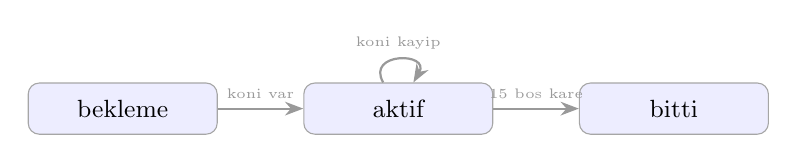
\begin{tikzpicture}[
  state/.style={rectangle, draw=gray!70, rounded corners=4pt,
                minimum width=2.4cm, minimum height=0.65cm,
                font=\small, text centered, fill=blue!7},
  arrow/.style={-Stealth, thick, gray!80}
]
\node[state] (bk) at (0,0)    {bekleme};
\node[state] (ak) at (3.5,0)  {aktif};
\node[state] (bt) at (7.0,0)  {bitti};

\draw[arrow] (bk) -- node[above]{\tiny koni var} (ak);
\draw[arrow] (ak) -- node[above]{\tiny 15 bos kare} (bt);
\draw[arrow] (ak) to[out=120,in=60,looseness=3]
             node[above]{\tiny koni kayip} (ak);
\end{tikzpicture}
\end{center}

\subsection{Gelismis Ozellikler}

\begin{description}[leftmargin=2em]
  \item[Baslangic kapisi] Iki koni simetrik gorulurse arac ikisi arasina
        hedeflenir (kapi mod).
  \item[Center weave] Koni tam merkezde ise hafif sallanma
        (amplitude 0.55) ile gecis saglanir.
  \item[S-weave] $\geq 6$ kare tek tarafta koni varsa S-sallanimli
        hareket uretilir (amplitude 0.45).
\end{description}

% ============================================================
\section{Park Mantigi (\texttt{parking\_logic.py})}
% ============================================================

\subsection{Amac}

Park alanina ulasildiktan sonra uygun slot bulup dik park manevrasi
gerceklestirmek icin bes asamali durum makinesi.

\begin{specbox}
Sartname: Dogru park $\to$ \textbf{80 puan}. Park girisinden
itibaren 3 dakika (180 s) icerisinde tamamlanmalidir.
\end{specbox}

\subsection{Park Faz Makinesi}

\begin{center}
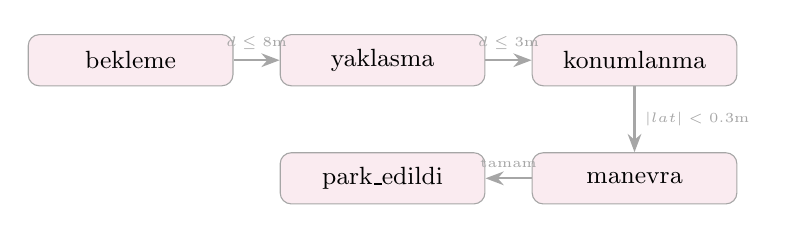
\begin{tikzpicture}[
  state/.style={rectangle, draw=gray!70, rounded corners=4pt,
                minimum width=2.6cm, minimum height=0.65cm,
                font=\small, text centered, fill=purple!8},
  arrow/.style={-Stealth, thick, gray!70}
]
\node[state] (w)  at (0,0)    {bekleme};
\node[state] (a)  at (3.2,0)  {yaklasma};
\node[state] (al) at (6.4,0)  {konumlanma};
\node[state] (m)  at (6.4,-1.5){manevra};
\node[state] (p)  at (3.2,-1.5){park\_edildi};

\draw[arrow] (w)  -- node[above]{\tiny $d\leq8$m} (a);
\draw[arrow] (a)  -- node[above]{\tiny $d\leq3$m} (al);
\draw[arrow] (al) -- node[right]{\tiny $|lat|<0.3$m} (m);
\draw[arrow] (m)  -- node[above]{\tiny tamam} (p);
\end{tikzpicture}
\end{center}

\begin{description}[leftmargin=2em]
  \item[bekleme] Park alani gorulmedi.
  \item[yaklasma] Slot goruldu ($d \leq 8$ m); hiz 0.40.
  \item[konumlanma] Lateral hizalama ($|lat| < 0{,}3$ m); hiz 0.20.
  \item[manevra] Geri giderek dik park; 20 kare onay sonrasi tamam.
  \item[park\_edildi] \texttt{complete=True}.
\end{description}

\subsection{Slot Secim Kurali}

\begin{center}
\begin{tabular}{ll}
  \toprule
  \texttt{parking\_allowed} & Davranis\\
  \midrule
  \texttt{True}  & Izinli slot: manevra hedefi olabilir\\
  \texttt{False} & Yasakli slot: kesinlikle secilmez\\
  \texttt{None}  & Belirsiz: gecilir, baska slot aranir\\
  \bottomrule
\end{tabular}
\end{center}

% ============================================================
\section{GPS / Waypoint Yoneticisi (\texttt{waypoint\_manager.py})}
% ============================================================

\subsection{Yonelim Hesaplari}

\textbf{Haversine mesafesi:}
\begin{equation}
  d = 2R \arctan\!\left(\frac{\sqrt{a}}{\sqrt{1-a}}\right),\;
  a = \sin^2\!\tfrac{\Delta\phi}{2} + \cos\phi_1\cos\phi_2\sin^2\!\tfrac{\Delta\lambda}{2}
\end{equation}

\textbf{Oncel azimut:}
\begin{equation}
  bearing = \arctan2\!\left(\sin\Delta\lambda\cos\phi_2,\;
            \cos\phi_1\sin\phi_2 - \sin\phi_1\cos\phi_2\cos\Delta\lambda\right)
\end{equation}

\textbf{Cross-track hatasi} (yoldan yatay sapma):
\begin{equation}
  xte = \arcsin\!\left(\sin\tfrac{d_{13}}{R}\cdot\sin(\theta_{13}-\theta_{12})\right)\cdot R
\end{equation}

\textbf{Direksiyon referansi:}
\begin{equation}
  steering = \text{clip}_{[-1,1]}\!\left(b_{err} \cdot \tfrac{1}{90} - xte \cdot \tfrac{1}{20}\right)
\end{equation}

\subsection{Varis Kosulu}

Standart varis:
\begin{equation}
  arrived = (dist \leq arrival\_radius\_m)
\end{equation}

\textbf{Pickup/Dropoff icin kafa acisi ek kosulu:}
\begin{equation}
  heading\_aligned = \bigl|\text{angle\_diff}(wp.heading\_deg,\; pos.heading\_deg)\bigr| \leq 30^\circ
\end{equation}
\begin{equation}
  arrived = dist\_ok \;\wedge\; heading\_aligned
\end{equation}

\begin{specbox}
Sartname: Yolcu alma/birakma noktasinda arac dogru kafa acisinda
olmalidir. Bu kontrol yalnizca \texttt{PICKUP/DROPOFF} + \texttt{heading\_deg}
tanimli waypoint'lerde uygulanir.
\end{specbox}

% ============================================================
\section{Gorev Yoneticisi (\texttt{mission\_manager.py})}
% ============================================================

\subsection{Amac}

\texttt{WaypointManager} ustune ince katman: pickup/dropoff bekleme,
park modu, zaman asimlari.

\begin{specbox}
Sartname: Yolcu alma/birakma bekleme suresi: 15--20 saniye (+70 p).
Park: 3 dakika icerisinde tamamlanmali.
\end{specbox}

\subsection{Hold (Bekleme) Mekanizmasi}

\begin{enumerate}
  \item Arac \texttt{PICKUP/DROPOFF} noktasina varir.
  \item \texttt{\_hold\_started\_at} kaydedilir.
  \item $elapsed < 15$ s: hiz tavan 0.0 (\texttt{hold\_remaining\_s > 0}).
  \item $elapsed \geq 15$ s: waypoint ilerlenir, \texttt{hold\_remaining\_s = 0}.
\end{enumerate}

\begin{warnbox}
\texttt{min\_hold = 15 s} ile arac en erken 15. saniyede ilerler.
\texttt{target\_hold = 20 s} yalnizca log icin; sistem hic 20 s'yi asmaz.
\end{warnbox}

\subsection{Park Modu}

\begin{itemize}
  \item \texttt{PARK\_ENTRY/PARK} noktasina varilinca \texttt{\_park\_active=True}.
  \item Hiz tavan 0.5; \texttt{park\_mode=True} sinyali gonderilir.
  \item \texttt{notify\_park\_completed()} cagirilinca waypoint ilerler.
  \item 180 s'de \texttt{park\_remaining\_s = 0}: zorunlu guvenli dur.
\end{itemize}

% ============================================================
\section{Karar Birlestirici (\texttt{decision\_arbiter.py})}
% ============================================================

\subsection{Birlesme Kurallari}

\begin{center}
\begin{tabular}{lll}
  \toprule
  Alan                     & Kural    & Aciklama\\
  \midrule
  \texttt{emergency\_stop} & OR       & Herhangi biri durursa sistem durur\\
  \texttt{speed\_cap}      & MIN      & En kisitlayici tavan kazanir\\
  \texttt{steer\_override} & PRIORITY & Asagidaki oncelik tablosuna gore\\
  \bottomrule
\end{tabular}
\end{center}

\subsection{Direksiyon Oncelik Tablosu}

\begin{center}
\begin{tabular}{clc}
  \toprule
  Oncelik & Kaynak (\texttt{name})    & Aciklama\\
  \midrule
  0       & \texttt{park}             & En yuksek: park manevrasi\\
  1       & \texttt{dynamic\_avoid}   & Dinamik engel kacmasi\\
  2       & \texttt{static\_avoid}    & Statik engel kacmasi\\
  3       & \texttt{slalom}           & Slalom manevrasi\\
  99      & (diger)                   & En dusuk oncelik\\
  \bottomrule
\end{tabular}
\end{center}

\subsection{Serit Kisiti (Lane Clamp)}

Avoidance tipi bir steer uretiyorsa ve gecerli \texttt{LaneBounds} varsa:

\begin{align}
  target\_y &= \pm 0{,}6 \text{ m}\\
  clamped\_y &= \text{clip}_{[right+margin,\; left-margin]}(target\_y)\\
  steer' &= steer \times \frac{|clamped\_y|}{|target\_y|}
\end{align}

Serit bilgisi yoksa ve \texttt{lane\_required\_for\_avoidance=True} ise
avoidance steer tamamen iptal edilir.

% ============================================================
\section{GeoJSON Gorev Okuyucu (\texttt{geojson\_mission\_reader.py})}
% ============================================================

\subsection{Desteklenen Gorev Tipleri}

\begin{center}
\begin{tabular}{lll}
  \toprule
  \texttt{TaskType}       & \texttt{task} alani & Esanlamlar (\texttt{name} alani)\\
  \midrule
  \texttt{START}          & start           & baslangic, basla\\
  \texttt{CHECKPOINT}     & checkpoint      & gorev, gorev\_1, tunel\\
  \texttt{STOP}           & stop            & durak, bus\_stop\\
  \texttt{PARK}           & park            & park\_yeri, otopark\\
  \texttt{PARK\_ENTRY}    & park\_entry     & park\_giris, otopark\_giris\\
  \texttt{PICKUP}         & pickup          & yolcu\_binimi, binis\\
  \texttt{DROPOFF}        & dropoff         & yolcu\_indirme, inis\\
  \bottomrule
\end{tabular}
\end{center}

\begin{notebox}
Gercek yaris GeoJSON'larinda \texttt{name} alani
\texttt{''gorev\_1''}, \texttt{''park\_giris''} gibi gelir;
\texttt{task} alani bos olabilir. Okuyucu bunu \texttt{name} ile telafi eder.
\end{notebox}

\subsection{Ozel Alanlar}

\begin{itemize}
  \item \texttt{heading\_deg}: Aracin o noktaya vardiginda olmasi gereken
        bas acisi ($0$--$360$, $\bmod 360$ ile normalize edilir).
  \item \texttt{speed\_limit\_ratio}: Noktaya ozel hiz kisiti ($0$--$1$).
  \item \texttt{radius\_m}: Varis kosulunu saglayan yaricap (varsayilan 3 m).
\end{itemize}

% ============================================================
\section{Cografi Yardimcilar (\texttt{geo\_utils.py})}
% ============================================================

Tek fonksiyon: \texttt{haversine\_m(lat1, lon1, lat2, lon2)} ---
WGS-84 kuresel yaklasiminda iki GPS koordinati arasindaki yuzey
mesafesini (metre) dondurur. $R = 6{,}371 \times 10^6$ m kullanilir.

% ============================================================
\section{Sartname Uyum Ozeti}
% ============================================================

\begin{center}
\renewcommand{\arraystretch}{1.2}
\begin{longtable}{p{5.0cm}ccp{4.0cm}}
  \toprule
  Sartname Gereksinimi   & Puan  & Modul                    & Durum\\
  \midrule
  \endhead
  Kirmizi isik ihlali    & $-30$ & traffic\_light\_logic     & Tam destek\\
  Yesil isik $\leq 5$ sn & $+40$ & traffic\_light\_logic     & Tam destek\\
  Yesil isik 5--30 sn    & $+20$ & traffic\_light\_logic     & Tam destek\\
  Yesil isik $>30$ sn    & $-20$ & traffic\_light\_logic     & Tam destek\\
  Tabela dogru tepki      & $+50$ & traffic\_sign\_logic      & 22/22 tabela\\
  Tabela yanlis tepki     & $-50$ & traffic\_sign\_logic      & Korunuyor\\
  Dinamik engel (yaya)    & $+50$ & obstacle\_logic           & Tam destek\\
  Statik engel            & $+50$ & obstacle\_logic           & Tam destek\\
  Serit ihlali            & $-50$ & decision\_arbiter         & Lane clamp\\
  Gorev noktasi ($\pm1$ m)& $+30$ & waypoint\_manager         & radius\_m=3 m\\
  Pickup/Dropoff          & $+70$ & mission\_manager          & 15--20 s bekleme\\
  Park                    & $+80$ & parking\_logic            & Tam durum mak.\\
  Tunel (opsiyonel)       &$+200$ & geojson\_mission\_reader  & Tercihli rota\\
  \bottomrule
\end{longtable}
\end{center}

\end{document}
